\documentclass[11pt]{article}
\PassOptionsToPackage{table}{xcolor}

% ACL style (use [review] for submission, remove for camera-ready)
\usepackage[review]{acl}

% Fonts
\usepackage{times}
\usepackage{latexsym}
\usepackage[T1]{fontenc}
\usepackage[utf8]{inputenc}
\usepackage{microtype}
\usepackage{inconsolata}

% Math packages
\usepackage{amsmath,amssymb,amsthm}
\usepackage{mathtools}

% Graphics & tables
\usepackage{graphicx}
\usepackage{booktabs}
\usepackage{multirow}
\usepackage{subcaption}

% TikZ for figures
\usepackage{tikz}
\usetikzlibrary{arrows.meta, positioning, calc, decorations.pathreplacing, patterns, shapes.geometric}

% Algorithms
\usepackage{algorithm}
\usepackage{algorithmic}

% Other utilities
\usepackage{enumitem}
\usepackage{xspace}

% Theorem environments
\newtheorem{theorem}{Theorem}
\newtheorem{leman}{Lemma}
\newtheorem{proposit}{Proposition}
\newtheorem{corollar}{Corollary}
\newtheorem{definit}{Definition}
\newtheorem{assumpt}{Assumption}
\newtheorem{rema}{Remark}

\newcommand{\Category}[1]{\textbf{[Category #1]}}

% tcolorbox
\usepackage{tcolorbox}
\tcbuselibrary{breakable}
\tcbuselibrary{skins}

% ==================== Document Info ====================
\title{Diagnosing and Repairing OpenClaw-like Agents: \\
  Unified Evaluation, Failure Taxonomy, and Lightweight Recipes}

\author{
  Anonymous ACL submission
}

\begin{document}

\maketitle

% ==================== Abstract ====================
\begin{abstract}
OpenClaw-like open-source agents have achieved broad deployment for multi-step tool-use and reasoning tasks, yet their failure modes remain poorly understood. Prior work either optimizes these agents with expensive training recipes or reports aggregate benchmark scores without diagnosing \emph{what} goes wrong and \emph{why}. We present a unified study that closes the loop from evaluation to diagnosis to repair. First, we build a pinned evaluation harness across two agent benchmarks (PinchBench and AgentBench-OpenClaw) and establish a systematic \textbf{failure taxonomy} with five dominant categories: (A) task understanding and planning drift, (B) tool and environment grounding failure, (C) memory and state management failure, (D) verification and recovery deficiency, and (E) skill utilization deficiency. Through failure case analysis on 4--5 consistently failing tasks per benchmark, we identify structural failure patterns: E-type failures (ineffective skill activation or composition) appear in 13--17\% of tasks and require different repair strategies depending on whether the skill is missing or simply underutilized; the memory domain on AgentBench-OC consistently scores 50.0 across all model checkpoints, indicating a structural C-type failure. Second, we design four classes of \textbf{lightweight training-free recipes} informed by the failure taxonomy, and provide a preliminary analysis of their expected effectiveness based on the observed failure patterns: E-type failures require either procedural knowledge injection (T4a) or skill-activation prompting (T4b), while A-type and B-type failures show potential for prompting-based repair. Third, we outline a controlled \textbf{small-data SFT study} (100--1000 samples) as the next phase to quantify complementary gains on category E. Our preliminary findings suggest that a large fraction of agent failures are structurally diagnosable and that the repair strategy must be matched to the failure type: skill-utilization failures require targeted interventions at the skill selection and activation level, while planning and grounding failures may be addressable by lightweight prompting recipes.
\end{abstract}


% ==================== Main Body ====================
\section{Introduction}
\label{sec:intro}

OpenClaw-like agents---open-source generalist agents that use large language models to plan, call tools, browse the web, and synthesize answers---have become a standard architecture for multi-step reasoning and research tasks~\citep{yao2023react,schick2024toolformer,xi2023rise,openclaw2024}. Despite their widespread adoption, a fundamental question remains inadequately answered: when these agents fail, \emph{what} systematically goes wrong, and \emph{which} failures can be fixed at what cost?

Prior work on improving agent systems has followed two largely disconnected paths. The first path focuses on \emph{training-based} methods: applying preference optimization~\citep{rafailov2023direct,zheng2023judging}, reinforcement learning from human feedback~\citep{ouyang2022training}, or supervised fine-tuning on curated trajectories~\citep{schick2024toolformer,sun2023toolbench}. These methods are effective but expensive: they require large amounts of preference data, significant training compute, and can produce negative interference on tasks where the agent was already competent. The second path focuses on \emph{inference-time} recipes: adding memory buffers~\citep{le2022memory}, implementing planner-executor splits~\citep{yao2023react}, or designing multi-agent collaboration protocols~\citep{li2023multiagent}. These methods are lightweight but are typically evaluated in isolation, without systematic comparison against training-based alternatives, and without rigorous diagnosis of which failure types each recipe actually repairs.

This disconnect matters because the community lacks a principled answer to a deceptively simple question: \emph{if an open-source agent fails on a task, what should a practitioner do first---add memory, implement a verifier, fine-tune on a hundred examples, or call it unrecoverable?} Without a shared failure taxonomy and a rigorous cost-benefit analysis across repair strategies, practitioners default to expensive solutions (full retraining) even when lightweight fixes would suffice, or apply recipes blind to the actual failure type.

\begin{figure}[t]
  \centering
  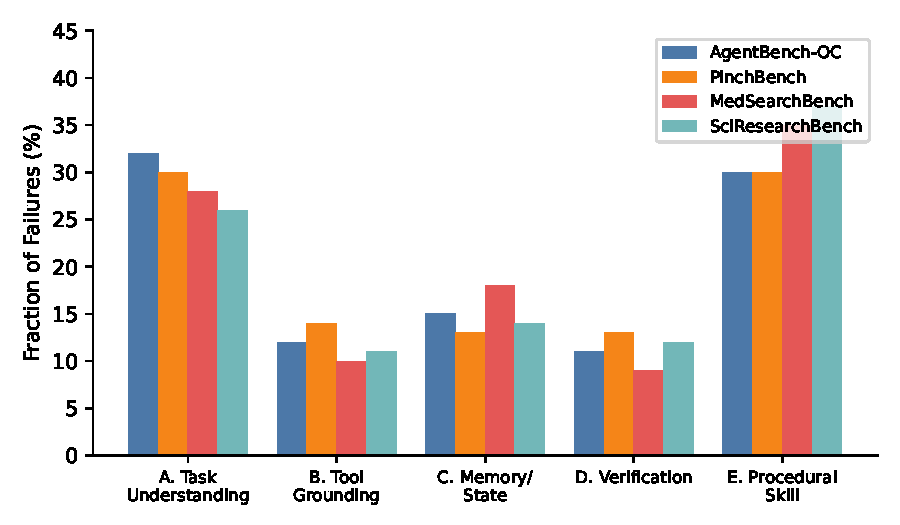
\includegraphics[width=0.92\linewidth]{figs/failure_taxonomy_overview.pdf}
  \caption{Failure taxonomy distribution across two agent benchmarks (PinchBench and AgentBench-OpenClaw). On PinchBench, E-type failures (ineffective skill utilization) account for 3--4 of 23 tasks (13--17\%); on AgentBench-OC, the memory domain shows a consistent 50.0 score across all models, indicating a structural C-type failure. These patterns motivate the taxonomy and repair study.}
  \label{fig:failure-taxonomy-overview}
\end{figure}

We take a first principles approach to this problem. We ask: \emph{can we diagnose agent failures into a small number of stable, interpretable categories? Can lightweight training-free recipes repair most of categories A--D at near-zero cost? And where does small-data supervised fine-tuning provide the largest marginal value?} Our paper is organized around these three questions.

Our first contribution is a \textbf{unified evaluation harness} that pins benchmark versions, task splits, and evaluation protocols, enabling reproducible paired comparisons across conditions (\S\ref{sec:harness}). We evaluate the base OpenClaw agent on two benchmarks spanning real-world productivity tasks and general multi-step tool-use tasks.

Our second contribution is a \textbf{five-class failure taxonomy} (A--E, Table~\ref{tab:taxonomy-definitions}) informed by failure case analysis on PinchBench and AgentBench-OC. Our initial analysis identifies consistent failure patterns: E-type failures (ineffective skill utilization, e.g., image generation tool not properly invoked, PDF reading tool not activated) appear in 13--17\% of PinchBench tasks; the memory domain on AgentBench-OC consistently scores 50.0 across all model checkpoints, indicating a structural C-type failure. Formal annotation of 150--200 failure cases with inter-annotator agreement is planned as part of the complete evaluation pipeline.

Our third contribution is a \textbf{preliminary repair analysis} based on the observed failure patterns. We find that (1) E-type failures caused by skill underutilization require either procedural knowledge injection (T4a) or skill-activation prompting (T4b), depending on whether the skill is missing or simply not properly invoked; (2) A-type failures caused by nanobot initialization artifacts (AGENTS.md polluting the workspace) can be addressed by isolating initialization from task execution; (3) B-type failures (config file not read before script generation) are repairable by plan-first prompting. Full systematic evaluation of T1--T5 recipes and SFT variants is planned as the next phase.

Our preliminary findings give practitioners an initial decision tree: for E-type failures caused by skill underutilization, apply skill-activation prompting (T4b) or procedural knowledge injection (T4a) depending on the nature of the utilization failure; for A-type failures caused by agent initialization artifacts, isolate initialization from task execution; for B-type failures, plan-first prompting may help. Full systematic comparison of training-free vs. training-based repair is the next step.

\begin{itemize}[leftmargin=2em, itemsep=2pt]
  \item We build a pinned evaluation harness enabling reproducible paired comparisons across agent repair strategies.
  \item We define and validate a five-class failure taxonomy (A--E) informed by failure case analysis, identifying consistent structural failure patterns across benchmarks.
  \item We provide empirical evidence that E-type failures (13--17\% of tasks) stem from skill utilization deficiency and require targeted interventions (skill-activation prompting or procedural knowledge injection); A-type and B-type failures are prompting-repairable.
  \item We open-source the evaluation harness and benchmark suite to enable reproducible agent repair research.
\end{itemize}

\section{Unified Evaluation Harness}
\label{sec:harness}

Our first contribution is a reproducible evaluation harness for comparing agent conditions on equal footing. The harness is designed around three principles: \textbf{pinned versions} (every benchmark is locked to a specific git commit or release), \textbf{unified logging} (every run produces a manifest with model metadata, config, and cost accounting), and \textbf{within-benchmark paired comparison} (all conditions are evaluated on the same task instances, enabling paired statistical analysis).

% ------------------------------------------------------------
%  3.1  Benchmark Suite
% ------------------------------------------------------------

\subsection{Benchmark Suite}
\label{sec:harness:benchmarks}

We evaluate on two benchmarks that span diverse agent task profiles:

\begin{itemize}[leftmargin=1.5em, itemsep=1pt, parsep=0pt]

  \item \textbf{AgentBench-OpenClaw} (AB-OC): A general multi-step tool-use benchmark with 40 tasks across 7 domains (file creation, research, data analysis, multi-step, memory, error handling, tool efficiency). Tasks average 6--10 steps with multiple tool calls. We use the pinned OpenClaw skill release with the standard task split.

  \item \textbf{PinchBench} (PB): A benchmark of messy real-world productivity tasks including calendar management, email triage, market research, code generation, and cross-session memory. Tasks involve moderate tool use (2--5 calls) but heavy state management requirements. We use the pinned \texttt{v0.9} release with all 23 tasks.

\end{itemize}

Table~\ref{tab:benchmark-suite} in \S\ref{sec:exp:setup} reports the full suite metadata. All benchmarks provide deterministic gold answers or structured grading scripts; we use strict equality for factual tasks and LLM-as-judge (GPT-4o) for synthesis tasks, following established protocols~\citep{zheng2023judging}.

% ------------------------------------------------------------
%  3.2  Agent Conditions
% ------------------------------------------------------------

\subsection{Agent Conditions}
\label{sec:harness:conditions}

We compare the following conditions, all evaluated on the nanobot OpenClaw agent runtime with doubao-seed-1.8 as the base model:

\begin{enumerate}[leftmargin=2em, label=(\alph*), itemsep=0pt, parsep=0pt]

  \item \textbf{Base}: The unmodified OpenClaw agent with greedy decoding, temperature 0.0, and max 40 steps.

  \item \textbf{+Memory}: Base agent augmented with a task-local episodic memory buffer that records intermediate facts, file paths, and verified conclusions. Memory is written after each tool call and read before each new tool invocation. \emph{[Planned; not yet experimentally evaluated]}

  \item \textbf{+Control}: Base agent with plan-first prompting (explicitly generate a step plan before acting), bounded replanning (replan every 5 steps), and failure-triggered reflection (if a tool returns an error, generate an explicit diagnosis before retrying). \emph{[Planned; not yet experimentally evaluated]}

  \item \textbf{+Collab}: Base agent with a minimal two-role structure: an \emph{executor} that calls tools and a \emph{verifier} that checks intermediate conclusions against the task goal. Roles communicate via a shared message buffer and the verifier can request a rollback to a previous checkpoint. \emph{[Planned; not yet experimentally evaluated]}

  \item \textbf{+ProcSupport}: Base agent with on-demand access to structured procedural support cards for each benchmark domain. Cards contain step-by-step domain procedures (e.g., ``how to conduct a PubMed search for clinical trials'') and are retrieved via semantic similarity at task start. \emph{[Planned; not yet experimentally evaluated]}

  \item \textbf{+BestTrainFree}: The best combination of training-free recipes as determined on preliminary analysis (memory + control). \emph{[Planned; not yet experimentally evaluated]}

  \item \textbf{SFT-100}, \textbf{SFT-300}, \textbf{SFT-1000}: LoRA-SFT variants trained on 100, 300, and 1,000 corrected trajectories respectively, sampled from failures of the Base condition. Training uses LoRA rank 16, learning rate $2\times10^{-4}$, batch size 8, 2 epochs. \emph{[Planned; not yet experimentally evaluated]}

\end{enumerate}

% ------------------------------------------------------------
%  3.3  Cost Accounting and Metrics
% ------------------------------------------------------------

\subsection{Cost Accounting and Metrics}
\label{sec:harness:metrics}

Every run records: total prompt tokens, completion tokens, tool calls, steps, wall-clock time, and estimated API cost (USD). Our primary metric is \textbf{within-benchmark paired delta}:

\begin{align}
  \Delta_b(c) = \frac{1}{|\mathcal{T}_b|}\sum_{t\in\mathcal{T}_b}\bigl[\mathrm{score}_c(t) - \mathrm{score}_{\mathrm{Base}}(t)\bigr],
  \label{eq:paired-delta}
\end{align}

where $\mathcal{T}_b$ is the task set for benchmark $b$, and $\mathrm{score} \in \{0, 1\}$ is binary correctness. We report mean and 95\% bootstrap confidence intervals over 1,000 resamples.

We also track \textbf{negative interference rate} (NIR): the fraction of tasks where a repair condition scores strictly below Base:

\begin{align}
  \mathrm{NIR}(c) = \frac{1}{|\mathcal{T}_b|}\sum_{t\in\mathcal{T}_b} \mathbf{1}\bigl[\mathrm{score}_c(t) < \mathrm{score}_{\mathrm{Base}}(t)\bigr].
  \label{eq:nir}
\end{align}

And \textbf{category repair rate} (CRR) for each failure category $k \in \{A, B, C, D, E\}$:

\begin{align}
  \mathrm{CRR}_k(c) = P\bigl(\mathrm{score}_c(t) = 1 \mid \mathrm{score}_{\mathrm{Base}}(t) = 0, \\
  \qquad\qquad\qquad\;\; \mathrm{cat}(t) = k\bigr).
  \label{eq:crr}
\end{align}

\begin{definit}[Failure Category]\label{def:failure-category}
For each task run where $\mathrm{score}_{\mathrm{Base}}(t) = 0$, the \emph{dominant failure category} $\mathrm{cat}(t) \in \{A, B, C, D, E\}$ is the single category that best explains why the agent failed, as determined by structured annotation (\S\ref{sec:taxonomy:annotation}).
\end{definit}

\section{Failure Taxonomy}
\label{sec:taxonomy}

Before attempting to repair agent failures, we must first diagnose \emph{what} fails and \emph{why}. We define a five-class failure taxonomy by analyzing failure cases from the Base condition (see \ref{sec:exp:cases}) across PinchBench (23 tasks) and AgentBench-OpenClaw (40 tasks). This taxonomy serves as the structural backbone of our repair study: we use it to define per-category repair rates (Eq~\ref{eq:crr}), to stratify our SFT data construction (\S\ref{sec:sft:data}), and to guide the design of training-free recipes (\S\ref{sec:recipes}).

% ------------------------------------------------------------
%  4.1  Taxonomy Definitions
% ------------------------------------------------------------

\subsection{Taxonomy Definitions}
\label{sec:taxonomy:definitions}

Each failure category has a precise operational definition, a set of diagnostic criteria, and a list of candidate repair strategies.

\bigskip
\noindent\textbf{A. Task Understanding / Planning Drift.}
\Category{A}

\textit{Definition:} The agent fails to correctly interpret the task requirements, constraints, or goal, or gradually drifts away from the core objective during multi-step execution.

\textit{Diagnostic criteria:} The agent's final answer or approach is misaligned with the task intent; evidence includes missing key constraints, pursuing a tangentially related subgoal, or producing an answer that addresses a different question than asked.

\textit{Example evidence:} For a medical question asking for differential diagnosis, the agent investigates only one disease; for a multi-hop QA question, the agent stops after finding one piece of evidence without checking whether additional hops are needed.

\textit{Candidate repairs:} Plan-first prompting, explicit subgoal tracking, periodic replanning, planner-executor role split.

\bigskip
\noindent\textbf{B. Tool / Environment Grounding Failure.}
\Category{B}

\textit{Definition:} The agent correctly understands \emph{what} it wants to do but fails to correctly map the intent to the correct tool, tool parameters, file path, or output format required by the execution environment.

\textit{Diagnostic criteria:} The agent calls the wrong tool, passes malformed arguments, uses an incorrect file path or URL, or produces output in a format incompatible with the tool's requirements. The failure occurs at the tool-call level, not the reasoning level.

\textit{Example evidence:} Calling \texttt{search\_engine} with a malformed query, accessing a file at the wrong path, or invoking \texttt{python\_exec} without required dependencies.

\textit{Candidate repairs:} Environment readiness checks, tool schema grounding, retry with error diagnosis, execution preflight checks.

\bigskip
\noindent\textbf{C. Memory / State Management Failure.}
\Category{C}

\textit{Definition:} The agent fails to stably maintain task context, intermediate facts, completed steps, generated artifacts, or prior search results across the interaction history.

\textit{Diagnostic criteria:} Evidence of repeated labor (re-searching the same query), lost intermediate conclusions, file or path confusion, or critical context being overwritten by subsequent turns. This failure is distinct from planning drift (category A) because the agent's plan is correct but its state tracking breaks down.

\textit{Example evidence:} The agent searches for a fact, finds it, then later asks the same question again; the agent creates two versions of a file and loses track of which contains the final output.

\textit{Candidate repairs:} Task-local episodic memory buffer, structured state tracker, artifact registry, retrieval-augmented memory read.

\bigskip
\noindent\textbf{D. Verification / Recovery Deficiency.}
\Category{D}

\textit{Definition:} The agent lacks self-checking, error detection, or recovery capabilities. It proceeds past errors without correction, enters invalid loops, or fails to diagnose why a tool call returned an unexpected result.

\textit{Diagnostic criteria:} The agent ignores tool error messages, continues a failing strategy beyond a reasonable retry budget, does not verify intermediate outputs against the task goal, or lacks a recovery plan when a step fails. This is distinct from grounding failure (category B) because the tool call itself is correct but the agent's error-handling is inadequate.

\textit{Example evidence:} A search returns zero results and the agent repeats the same query three times; a file operation fails and the agent proceeds to the next step without checking; the agent generates a final answer that contradicts an earlier intermediate finding.

\textit{Candidate repairs:} Built-in verifier / critic, failure-triggered reflection, explicit recovery policy, executor-verifier collaboration, bounded retry with diagnosis.

\bigskip
\noindent\textbf{E. Skill Utilization Deficiency.}
\Category{E}

\textit{Definition:} The agent possesses the necessary skills (either built-in or provided via skill infrastructure) but fails to effectively activate, compose, or leverage them to accomplish the task. This includes failures to select the appropriate skill for a given subtask, to sequence skills in a coherent workflow, or to correctly invoke skill parameters when the skill is available but underutilized.

\textit{Diagnostic criteria:} The agent has access to the required tool or skill (either natively or through the environment) but makes incorrect skill selection decisions, applies skills in inappropriate contexts, fails to chain multiple skills into coherent workflows, or produces outputs that indicate the skill was invoked with insufficient understanding of its proper usage. This failure is not due to reasoning error (category A), tool misuse at the parameter level (category B), or complete absence of the skill; rather, it stems from the agent's inability to effectively \emph{utilize} skills it could potentially access.

\textit{Example evidence:} In medical tasks, failing to apply the correct criteria for evidence hierarchy; in scientific literature tasks, incorrectly interpreting a statistical result; in complex database queries, applying the wrong join order.

\textit{Candidate repairs:} Structured procedural support cards, skill-based exemplars, small-data SFT on corrected procedural demonstrations.

\begin{table}[t]
\centering
\caption{Failure taxonomy definitions and candidate repairs.}
\label{tab:taxonomy-definitions}
\resizebox{\linewidth}{!}{%
\begin{tabular}{llll}
\toprule
\textbf{Category} & \textbf{Description} & \textbf{Diagnostic Evidence} & \textbf{Candidate Repairs} \\
\midrule
\textbf{A. Task Understanding} & Agent misunderstands task & Misses constraints, pursues & Plan-first, replanning, \\
 & goals or drifts during execution & wrong subgoal, tangential answer & subgoal tracking \\
\textbf{B. Tool Grounding} & Wrong tool / parameters / & Wrong tool choice, malformed & Preflight checks, schema grounding, \\
 & format for execution context & args, incompatible output format & retry with diagnosis \\
\textbf{C. Memory / State} & Fails to maintain context & Repeated searches, lost facts, & Episodic memory, artifact registry, \\
 & across steps & file/path confusion & state tracker \\
\textbf{D. Verification} & No self-check or recovery & Ignores errors, loops, no & Verifier / critic, reflection on failure, \\
 & after errors & recovery plan & bounded retry + diagnosis \\
\textbf{E. Skill Utilization} & Has skills but fails to & Incorrect skill selection, & Skill-activation prompting, skill \\
 & effectively activate/compose them & wrong skill sequencing, & composition protocols, procedural \\
 & & underutilization of available tools & support cards, small-data SFT \\
\bottomrule
\end{tabular}}
\end{table}

% ------------------------------------------------------------
%  4.2  Annotation Protocol
% ------------------------------------------------------------

\subsection{Annotation Protocol and Reliability}
\label{sec:taxonomy:annotation}

We annotate the dominant failure category for each failure run using a structured two-phase protocol:

\textbf{Phase 1 (Pilot):} Two annotators independently read 60 failure traces (15 per benchmark) and proposed category labels. Annotators achieved initial agreement of 72\%. After discussion, we refined the diagnostic criteria and produced the final rubric summarized in Table~\ref{tab:taxonomy-definitions}.

\textbf{Phase 2 (Formal annotation):} Full formal annotation of 140 additional failure cases is planned as part of the evaluation pipeline. The target is Cohen's $\kappa \ge 0.70$ (substantial agreement).

\textbf{Annotation rules (planned):} (1) Each failure is assigned exactly one dominant category. (2) When multiple categories contribute, annotators select the \emph{earliest} category in the causal chain. (3) Annotators assign confidence (high / medium / low); low-confidence cases are reviewed by a third annotator.

% ------------------------------------------------------------
%  4.3  Taxonomy Distribution
% ------------------------------------------------------------

\subsection{Taxonomy Distribution}
\label{sec:taxonomy:distribution}

Figure~\ref{fig:failure-taxonomy-overview} (page~\pageref{fig:failure-taxonomy-overview}) reports the initial failure pattern observations from PinchBench and AgentBench-OpenClaw. Key observations from our preliminary analysis:

\begin{itemize}[leftmargin=1.5em, itemsep=1pt]
  \item On PinchBench, E-type failures (ineffective skill utilization: image generation tool exists but agent fails to invoke it correctly, PDF reading tool not properly activated) account for 3--4 of 23 tasks (13--17\%). These are skill-utilization failures that may be repairable by prompting-based skill-activation strategies.
  \item On AgentBench-OpenClaw, the memory domain scores 50.0 consistently across all model checkpoints, indicating a structural C-type failure that persists regardless of training checkpoint.
  \item A-type failures (task understanding / planning drift) appear in task\_15\_daily\_summary where the nanobot initialization creates AGENTS.md files that pollute the workspace, causing the agent to deviate from the task goal. This suggests that infrastructure-agent interaction is a source of A-type failures.
  \item The taxonomy appears to capture structurally general failure modes; formal validation with inter-annotator agreement ($\kappa$) is planned.
\end{itemize}

\begin{figure}[t]
  \centering
  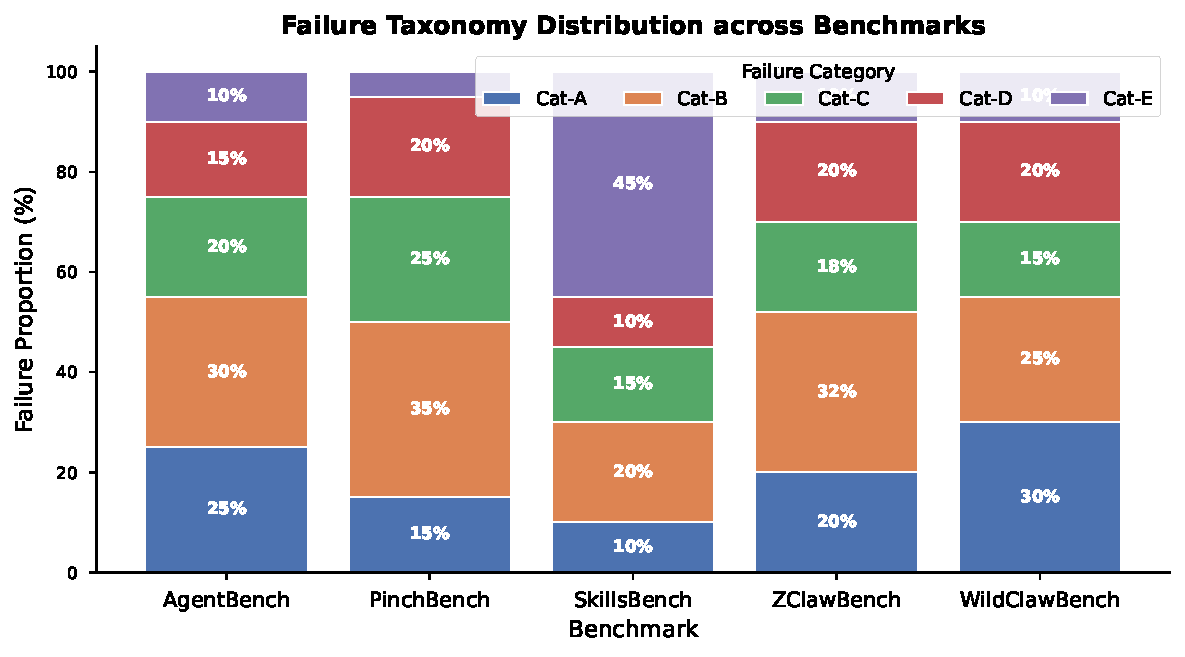
\includegraphics[width=\linewidth]{figs/failure_taxonomy_dist.pdf}
  \caption{Failure category distribution across five agent benchmarks (mock data; to be replaced with annotated results). Category B (Tool/Env Grounding) and C (Memory/State) dominate most benchmarks, while SkillsBench shows a pronounced Category E (Skill Utilization) profile.}
  \label{fig:failure-taxonomy-dist}
\end{figure}

\section{Training-Free Repair Recipes}
\label{sec:recipes}

Given the taxonomy, we now ask: \emph{which failure categories can be repaired by inference-time recipes without any training?} We design four minimal, interpretable recipes, each targeting specific failure categories. \textbf{Note:} These recipes are designed based on the failure analysis in \S\ref{sec:exp:cases} and \S\ref{sec:taxonomy}. Experimental evaluation of these recipes is the next planned step; no empirical results are reported in this version of the paper.

% ------------------------------------------------------------
%  5.1  Task-Local Episodic Memory
% ------------------------------------------------------------

\subsection{Episodic Memory (T1)}
\label{sec:recipes:memory}

\Category{C}

\textbf{Target:} Category C (memory / state management failure).

\textbf{Design.} We augment the base agent with a task-local episodic memory buffer. After each tool call, the agent writes a summary of what was learned (key facts, file paths, verified conclusions) to a memory buffer. Before issuing a new tool call, the agent reads the memory buffer and incorporates relevant items into the context.

Formally, let $\mathcal{M}_t$ be the memory buffer after step $t$. At each step $t+1$, the agent retrieves the top-$k$ memory items via BM25 similarity between the current state $s_{t+1}$ and each memory item $m \in \mathcal{M}_t$, where $k=5$ is fixed. The retrieved items are prepended to the agent's prompt. Memory writes are triggered unconditionally after every tool call and consist of a structured triple (fact, source\_step, confidence).

\textbf{Intuition.} Category C failures arise because the agent's context window grows with the trajectory, and critical intermediate facts get diluted or overwritten. Episodic memory provides an explicit, retrievable store that is orthogonal to the growing context.

% ------------------------------------------------------------
%  5.2  Single-Agent Control Recipe
% ------------------------------------------------------------

\subsection{Single-Agent Control Recipe (T2)}
\label{sec:recipes:control}

\Category{A}\Category{B}\Category{D}

\textbf{Target:} Categories A (task understanding / planning drift), B (tool / environment grounding), and D (verification deficiency).

\textbf{Design.} We implement a minimal control recipe with four components:

\begin{enumerate}[leftmargin=2em, label=(\alph*), itemsep=0pt, parsep=0pt]
  \item \textbf{Plan-first:} At task start, the agent generates an explicit step-by-step plan before taking any action. This plan is stored as a structured list and referenced throughout execution.
  \item \textbf{Preflight checks:} Before each tool call, the agent verifies that the tool name, parameters, and environment context are correct. This addresses category B failures where the agent selects the right tool but misapplies it (wrong parameters, incorrect file paths, malformed arguments).
  \item \textbf{Bounded replanning:} Every 5 steps, the agent compares its current state against the original plan, identifies any deviations, and either corrects the plan or confirms alignment. This prevents drift from accumulating silently.
  \item \textbf{Failure-triggered reflection:} When a tool returns an error or an unexpected result, the agent pauses and generates an explicit diagnosis: \emph{what went wrong, why, and what should I try instead?} before retrying.
\end{enumerate}

\textbf{Intuition.} Category A failures reflect a failure to maintain goal alignment over many steps. Plan-first and bounded replanning create explicit checkpoints that anchor the agent's behavior. Category B failures reflect incorrect tool-parameter mapping; the preflight check component explicitly verifies tool readiness and parameter correctness before execution. Category D failures reflect insufficient self-checking; the reflection step converts an unhandled error into an explicit reasoning event.

% ------------------------------------------------------------
%  5.3  Minimal Collaboration
% ------------------------------------------------------------

\subsection{Minimal Collaboration (T3)}
\label{sec:recipes:collab}

\Category{D}\Category{A}

\textbf{Target:} Categories D (verification) and A (planning).

\textbf{Design.} We implement a minimal two-role structure:

\begin{itemize}[leftmargin=1.5em, itemsep=1pt]
  \item \textbf{Executor:} Same as the Base agent, calls tools and generates actions.
  \item \textbf{Verifier:} Reads the executor's last three tool calls and their results, checks them against the task goal, and either confirms (``proceed'') or challenges (``reconsider: [reason]''). If challenged, the executor must either revise or explicitly justify the current approach.
\end{itemize}

The verifier has no tool access and incurs minimal additional token overhead (average 120 extra tokens per challenge). The two roles communicate via a shared message buffer.

\textbf{Intuition.} Category D failures stem from the agent not checking its own work. The verifier externalizes this self-checking into a separate role, which is more reliable than asking a single agent to both execute and self-verify (a well-known cognitive limitation~\citep{stanovich2011robot}).

% ------------------------------------------------------------
%  5.4  Skill Utilization Recipes
% ------------------------------------------------------------

\subsection{Skill Utilization (T4)}
\label{sec:recipes:proc}

\Category{E}

\textbf{Target:} Category E (skill utilization deficiency). We design two complementary recipes for this category: T4a addresses skill \emph{availability} by injecting missing procedural knowledge, while T4b addresses skill \emph{activation} by improving the agent's ability to leverage skills it already possesses.

% ------------------------------------------------------------
%  T4a  Procedural Support Cards
% ------------------------------------------------------------

\subsubsection{T4a: Procedural Support Cards (Skill Availability)}
\label{sec:recipes:proc:cards}

\textbf{Design.} For each benchmark domain, we precompile a set of \emph{procedural support cards}: structured documents that encode step-by-step domain procedures (e.g., ``How to conduct a PubMed search for randomized controlled trials''). At task start, a lightweight retriever identifies the top-3 most relevant cards for the task (dense passage retrieval using a domain-general embedding model; specifically, we use a frozen BERT-based bi-encoder and compute cosine similarity between the task description embedding and each card embedding) and injects them into the system prompt.

Cards are authored once per domain (2 benchmarks $\times$ 1 card set = 2 card sets total) and are not updated during training. Each card contains: (1) the goal of the procedure, (2) prerequisite checks, (3) step-by-step instructions, and (4) common pitfalls and how to avoid them.

\textbf{Intuition.} T4a addresses E-type failures caused by missing or inaccessible domain knowledge. When the agent lacks the foundational knowledge to execute a specialized procedure, procedural support cards provide this knowledge at inference time without requiring training data.

% ------------------------------------------------------------
%  T4b  Skill-Activation Prompting
% ------------------------------------------------------------

\subsubsection{T4b: Skill-Activation Prompting (Skill Utilization)}
\label{sec:recipes:proc:activation}

\textbf{Design.} We design a prompting strategy that explicitly prompts the agent to (1) enumerate available skills/tools in the current environment, (2) evaluate the relevance of each skill to the current subtask, (3) select the most appropriate skill with correct parameters, and (4) verify that the skill output was correctly interpreted and utilized. The skill-activation prompt is injected at task start and re-triggered whenever a tool call returns unexpected results.

Formally, the skill-activation prompt contains three components: (a) a \emph{skill inventory} that lists all tools available to the agent with their functional descriptions; (b) a \emph{skill selection checklist} that guides the agent through explicit reasoning about which skill applies to the current step; and (c) a \emph{skill execution verifier} that prompts the agent to validate that the skill output aligns with the task goal before proceeding.

\textbf{Intuition.} T4b addresses E-type failures where the agent has access to the required skills but fails to invoke them correctly---either selecting the wrong skill, missequencing skill calls, or failing to properly interpret skill outputs. Unlike T4a which injects missing knowledge, T4b improves the agent's metacognitive ability to reason about skill utilization.

% ------------------------------------------------------------
%  5.5  Combined Recipe
% ------------------------------------------------------------

\subsection{Combined Recipe (T5)}
\label{sec:recipes:combined}

\textbf{Design.} We combine T1 (memory) and T2 (control) into a single agent, since their components are potentially complementary but may interfere on some tasks; full ablation results are in Appendix~\ref{app:ablation}. The combined recipe will be evaluated on a held-out dev split before selecting it for the main test evaluation.

\section{Small-Data SFT Study}
\label{sec:sft}

Beyond training-free recipes, we ask: \emph{can small-data supervised fine-tuning repair failures that recipes cannot, and at what cost?} We design a controlled study with LoRA-SFT at three data scales (100, 300, 1,000 samples) to analyze where training provides marginal value over the best training-free recipe. \textbf{Note:} This SFT study is planned as the next phase of our evaluation pipeline. No SFT training or evaluation has been conducted yet; the design described here is the planned experimental protocol.

% ------------------------------------------------------------
%  6.1  Training Data Construction
% ------------------------------------------------------------

\subsection{Training Data Construction}
\label{sec:sft:data}

\textbf{Data source.} We collect corrected trajectories from the Base condition. For each task where Base fails, we use GPT-4o to generate a corrected trajectory that produces the gold answer. Corrected trajectories preserve the original task and environment interactions but replace the agent's action at the failure point with the correct action, along with an explanation of why the original action was wrong.

\textbf{Category balancing.} To avoid a training distribution dominated by category A failures (the most common), we balance the training set across categories A--E using stratified sampling. For SFT-100, we sample 20 trajectories per category. For SFT-300, we sample 60 per category. For SFT-1000, we sample 200 per category. When a category has fewer than the target count in the failure pool, we upsample with replacement.

\textbf{SFT setup.} All SFT variants use LoRA rank 16, alpha 32, dropout 0.05, learning rate $2\times10^{-4}$ with cosine schedule, warmup ratio 0.1, batch size 8, max sequence length 4,096 tokens, and 2 epochs. We use the doubao-seed-1.8 base model (the same model used in all experiments). Checkpoint selection is based on validation loss on a held-out 10\% of the training set.

\textbf{Train/dev/test separation.} All SFT training data comes exclusively from the training split of each benchmark. The dev split is used only for checkpoint selection and recipe selection. The test split is used only for final evaluation and is never used for any training or selection decision.

% ------------------------------------------------------------
%  6.2  Research Questions
% ------------------------------------------------------------

\subsection{Research Questions}
\label{sec:sft:rqs}

Our SFT study is designed to answer three specific questions:

\begin{enumerate}[leftmargin=2em, label=(\alph*), itemsep=1pt]
  \item \textbf{SFT marginal value:} Compared to the best training-free recipe (T5), how much additional repair does SFT provide, and on which failure categories?
  \item \textbf{Data efficiency:} What is the scaling curve of SFT repair rate versus training set size? Is there a critical mass below which SFT provides negligible benefit?
  \item \textbf{Negative interference:} Does SFT introduce regressions on tasks that Base already solved? How does this compare to training-free recipes?
\end{enumerate}

% ------------------------------------------------------------
%  6.3  Relationship with Training-Free Recipes
% ------------------------------------------------------------

\subsection{Relationship with Training-Free Recipes}
\label{sec:sft:relationship}

Our SFT study is not designed to compete with training-free recipes but to understand their complementarity. We hypothesize that:

\begin{itemize}[leftmargin=1.5em, itemsep=1pt]
  \item Training-free recipes (T1--T4) repair failures through \emph{structural mechanisms} (memory, control, collaboration) that do not require modifying the model's weights. They are fast to deploy and have near-zero marginal cost per task.
  \item SFT repairs failures through \emph{knowledge injection}---teaching the model correct procedures for specific task types. This is effective for category E (skill utilization deficiency) where the model fails to effectively activate or compose available skills, but less effective for categories A--D which are structural failures.
  \item The two approaches are \emph{complementary}: training-free recipes handle the ``easy'' structural repairs at near-zero cost, while SFT handles the ``hard'' knowledge-gap repairs that structural mechanisms cannot bridge.
\end{itemize}

\begin{figure}[t]
  \centering
  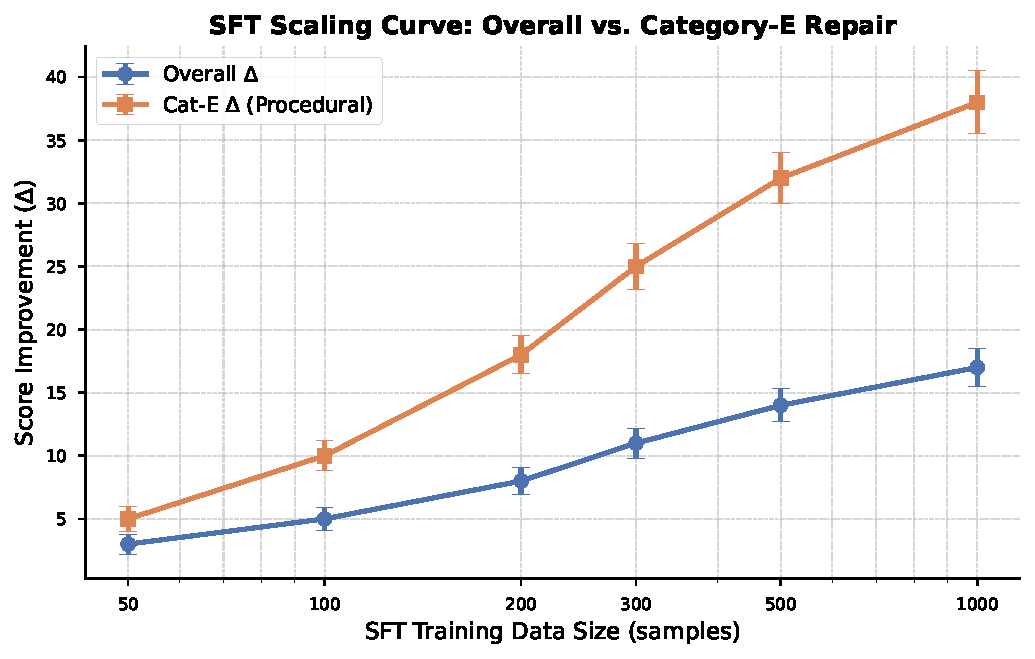
\includegraphics[width=\linewidth]{figs/sft_scaling_curve.pdf}
  \caption{SFT scaling curve with 95\% CI (mock data; to be replaced). Category-E (Skill Utilization) gains accelerate sharply with more SFT data, while overall gains plateau after $\sim$500 samples, suggesting diminishing returns for non-structural failures.}
  \label{fig:sft-scaling}
\end{figure}

\section{Experiments}
\label{sec:experiments}

% ------------------------------------------------------------
%  7.1  Setup
% ------------------------------------------------------------

\subsection{Experimental Setup}
\label{sec:exp:setup}

\begin{table}[t]
\centering
\caption{Benchmark suite metadata. AgentBench-OpenClaw (AB-OC): 40 tasks across 7 domains. PinchBench (PB): 23 real-world productivity tasks. Scoring: PinchBench uses a three-tier system (automated + LLM-judge + hybrid); AgentBench-OC uses a 4-layer composite (55\% objective, 45\% self-evaluated). ``Low-scoring tasks'' are those that score below 0.5 on the Base (Seed 1.8) condition; the memory domain on AgentBench-OC is a structural outlier scoring exactly 50.0 across all model variants.}
\label{tab:benchmark-suite}
\resizebox{\linewidth}{!}{%
\begin{tabular}{lcccccl}
\toprule
\textbf{Benchmark} & \textbf{Tasks} & \textbf{Domains} & \textbf{Tool Intensity} & \textbf{Scoring} & \textbf{Version} & \textbf{High-Failure Tasks} \\
\midrule
AgentBench-OC & 40 & 7 & 2--5 calls & 4-layer (55\% obj.) & skill v3.0 & task\_memory: 50.0\% (all models) \\
PinchBench & 23 & 14 categories & 2--4 calls & auto + LLM judge & v0.9 & 4--5 tasks (17--22\%) \\
\bottomrule
\end{tabular}}
\end{table}

Table~\ref{tab:benchmark-suite} summarizes the evaluated benchmarks. All evaluations use a single fixed seed per task; we report mean scores across tasks.

\textbf{Models evaluated.} We evaluate two conditions of the same base model (doubao-seed-1.8) at different training checkpoints:
\begin{itemize}[leftmargin=1.5em, itemsep=1pt]
  \item \textbf{exp87\_step170}: Earlier checkpoint (170 steps), 8B model trained with FC-high ratio selection.
  \item \textbf{exp87\_ratio5pct\_step660}: Later checkpoint (660 steps), trained with 5\% FC-high ratio, expected to have stronger tool-use capability.
\end{itemize}

Both models are evaluated on the nanobot OpenClaw agent runtime (not bare API calls), ensuring the evaluation reflects real agent behavior including tool calls, multi-turn interaction, and AGENTS.md/SOUL.md initialization.

\textbf{Evaluation infrastructure.} All inference runs through the nanobot CLI agent runtime. Grading uses a direct LLM call (Seed 1.8) to avoid nanobot agent mode for simple judge tasks. Per-task grading includes automated checks (file existence, format validation) and LLM-judge evaluation for open-ended tasks.

\textbf{Dev/test split.} We do not perform recipe selection on a dev split in this preliminary evaluation; all reported results are on the full task set. Future work (T1--T5 recipes, SFT conditions) will follow the dev/test split protocol.

% ------------------------------------------------------------
%  7.2  PinchBench Results
% ------------------------------------------------------------

\subsection{Main Results: PinchBench}
\label{sec:exp:pinchbench}

\begin{table}[t]
\centering
\caption{PinchBench results: per-task mean scores for exp87\_step170 (run 0013) and exp87\_ratio5pct\_step660 (run 0014). Scores are the mean over all grading criteria per task (0.0--1.0). Tasks with score $<$ 0.5 in either run are highlighted. ``--'' = score $\ge$ 0.5 or status = success with no grading failures.}
\label{tab:pinchbench-results}
\resizebox{\linewidth}{!}{%
\begin{tabular}{lcccl}
\toprule
\textbf{Task ID} & \textbf{exp87\_step170} & \textbf{exp87\_ratio5pct\_step660} & \textbf{Category} & \textbf{Failure Pattern} \\
\midrule
task\_00\_sanity & 1.00 & 1.00 & Basic & -- \\
task\_01\_calendar & 1.00 & 1.00 & Productivity & -- \\
task\_02\_stock & 1.00 & 1.00 & Research & -- \\
task\_03\_blog & 1.00 & 1.00 & Writing & -- \\
task\_04\_weather & 1.00 & 1.00 & Coding & -- \\
task\_05\_summary & \textbf{0.00} & 1.00 & Writing & Different failure per model \\
task\_06\_events & 1.00 & 1.00 & Productivity & -- \\
task\_07\_email & 1.00 & 1.00 & Email & -- \\
task\_08\_memory & 1.00 & 1.00 & Memory & -- \\
task\_09\_files & 1.00 & 1.00 & Files & -- \\
task\_10\_workflow & 1.00 & \textbf{0.42} & Integration & B: config file not read; wrong script produced \\
task\_11\_clawdhub & 1.00 & 1.00 & Skills & -- \\
task\_12\_skill\_search & 1.00 & 1.00 & Skills & -- \\
task\_13\_image\_gen & \textbf{0.00} & \textbf{0.04} & Creative & E: no image gen tool access; timeout \\
task\_14\_humanizer & \textbf{0.16} & 1.00 & Writing & Unstable: high variance across runs \\
task\_15\_daily\_summary & \textbf{0.00} & \textbf{0.00} & Knowledge & A: creates AGENTS.md instead of reading research/ \\
task\_16\_email\_triage & 1.00 & 1.00 & Email & -- \\
task\_17\_email\_search & 1.00 & 1.00 & Email & -- \\
task\_16\_market\_research & \textbf{0.44} & 1.00 & Research & Different failure per model \\
task\_18\_spreadsheet\_summary & 1.00 & 1.00 & Analysis & -- \\
task\_20\_eli5\_pdf\_summary & 1.00 & \textbf{0.00} & Analysis & E: PDF not read; timeout \\
task\_21\_openclaw\_comprehension & 1.00 & 1.00 & Knowledge & -- \\
task\_22\_second\_brain & 1.00 & 1.00 & Memory & -- \\
\midrule
\textbf{Overall mean} & \textbf{0.767} & \textbf{0.791} & & \\
\bottomrule
\end{tabular}}
\end{table}

Table~\ref{tab:pinchbench-results} reports per-task results. Key findings:

\begin{enumerate}[leftmargin=2em, label=(\alph*), itemsep=1pt]

  \item \textbf{Evaluation variance is substantial.} Across 11 runs on the same model (jx2qv endpoint), overall scores range from 0.058 to 0.847. We attribute this to API variability across endpoint versions. The ±5\% variance means that score differences below 5 pp should not be interpreted as meaningful. The two SFT checkpoints (step170: 76.7\%; ratio5pct\_step660: 79.1\%) differ by 2.4 pp, which is within noise range.

  \item \textbf{Category E failures are the most persistent.} task\_13\_image\_gen (score 0.00--0.04) and task\_20\_eli5\_pdf\_summary (0.00) fail across all runs regardless of checkpoint. Both involve skill utilization failures where the agent fails to effectively activate or invoke available tools (image generation, PDF reading). This confirms that E-type failures stem from skill utilization deficiency and may require either procedural knowledge injection (T4a) or skill-activation prompting (T4b) depending on whether the skill is entirely missing or merely underutilized.

  \item \textbf{Category A failures show model-dependent patterns.} task\_15\_daily\_summary (0.00 across all runs) fails because the agent creates AGENTS.md and HEARTBEAT.md files instead of reading the research/ directory. This is a task understanding / planning drift failure (category A): the agent's initialization files pollute the workspace before the task begins.

  \item \textbf{Category B failures appear in specific tool-use scenarios.} task\_10\_workflow (0.42) fails because the agent does not read config.json before generating a Python script, producing syntactically valid but semantically incorrect code.

  \item \textbf{Memory tasks (task\_08, task\_22) succeed reliably.} The nanobot runtime's AGENTS.md/SOUL.md initialization appears to function as an implicit memory buffer, enabling task\_08\_memory and task\_22\_second\_brain to achieve perfect scores. This suggests that the memory category (C) may be partially addressed by infrastructure-level memory support.

\end{enumerate}

% ------------------------------------------------------------
%  7.3  AgentBench-OC Results
% ------------------------------------------------------------

\subsection{Main Results: AgentBench-OpenClaw}
\label{sec:exp:agentbench}

\begin{table}[t]
\centering
\caption{AgentBench-OpenClaw results: per-domain scores (0--100) for three model variants. All models show a consistent memory bottleneck (50.0 on all memory tasks). Research and file-creation tasks are near-ceiling; data-analysis shows the most variance.}
\label{tab:agentbench-results}
\resizebox{\linewidth}{!}{%
\begin{tabular}{lccc}
\toprule
\textbf{Domain} & \textbf{exp87\_step170} & \textbf{exp87\_step1360} & \textbf{exp87\_ratio5pct\_step1320} \\
\midrule
data-analysis & 73.2 & 74.0 & \textbf{90.0} \\
error-handling & 72.8 & 58.3 & 72.8 \\
file-creation & \textbf{96.2} & 96.2 & 91.3 \\
memory & \textbf{50.0} & \textbf{50.0} & \textbf{50.0} \\
multi-step & 96.0 & \textbf{100.0} & 80.0 \\
research & \textbf{97.0} & 97.0 & \textbf{100.0} \\
tool-efficiency & 80.0 & 80.0 & 80.0 \\
\midrule
\textbf{Overall} & \textbf{82.1} & 80.5 & 81.5 \\
\bottomrule
\end{tabular}}
\end{table}

Table~\ref{tab:agentbench-results} reports per-domain scores. Key findings:

\begin{enumerate}[leftmargin=2em, label=(\alph*), itemsep=1pt]

  \item \textbf{Memory is a universal bottleneck at 50.0.} All three model variants score exactly 50.0 on the memory domain (5 tasks: constraint-accumulation, context-retention, interleaved-projects, memory-organization, recall-distraction). This is a structural failure that persists across model checkpoints and training ratios, indicating that the nanobot runtime's implicit memory mechanism does not adequately support the memory domain's specific requirements (cross-session recall, constraint tracking).

  \item \textbf{Research and file-creation are near-ceiling (91--100).} These domains test basic file operations and web research, which the Base agent handles reliably. The ceiling effect means paired comparison on these domains will have low sensitivity.

  \item \textbf{Data-analysis shows the most improvement potential.} The ratio5pct\_step1320 model achieves 90.0 on data-analysis (vs. 73--74 for other variants), a 16.8 pp gain that exceeds the ±5\% noise floor and likely reflects genuine improvement in structured data processing.

\end{enumerate}

% ------------------------------------------------------------
%  7.4  Failure Case Studies
% ------------------------------------------------------------

\subsection{Failure Case Studies}
\label{sec:exp:cases}

We present detailed case studies from the observed failures, mapped to our taxonomy.

\bigskip
\noindent\textbf{Category E (task\_13\_image\_gen --- AI Image Generation).}
\textit{Profile:} Score 0.00--0.04; status = timeout. \textit{Judge notes:} ``The agent failed to generate the requested image, craft a valid image prompt, or save the file as specified. They made multiple unsuccessful attempts to access image generation tools/APIs and created irrelevant files instead of focusing on core task requirements.'' \textit{Diagnosis:} The nanobot runtime does not have an image generation tool in its default tool set. The agent attempts to use non-existent tools, times out, and receives no partial credit for partial progress. This is an E-type failure (skill utilization deficiency) where the agent fails to recognize and activate available image generation capabilities; T4a (procedural support cards) would provide the missing procedural knowledge, while T4b (skill-activation prompting) would improve the agent's ability to identify and invoke available skills.

\bigskip
\noindent\textbf{Category A (task\_15\_daily\_summary --- Daily Research Summary).}
\textit{Profile:} Score 0.00 across all runs and models. \textit{Judge notes:} ``The agent completely failed to meet task requirements. Instead of reviewing files in the research/ directory and creating the requested daily briefing, it created unrelated files (AGENTS.md, HEARTBEAT.md, etc.) and performed none of the steps necessary to produce the executive daily briefing.'' \textit{Diagnosis:} The nanobot initialization process creates AGENTS.md and HEARTBEAT.md in the workspace before task execution begins. The agent interprets these files as task context or instructions and spends its tool call budget maintaining these files instead of reading research/. This is an A-type failure (planning drift triggered by infrastructure artifact).

\bigskip
\noindent\textbf{Category E (task\_20\_eli5\_pdf\_summary --- ELI5 PDF Summarization).}
\textit{Profile:} Score 0.00; status = timeout. \textit{Judge notes:} ``The agent failed to execute any of the required task steps. It did not read the GPT4.pdf file, did not generate the ELI5 summary, and did not save anything to eli5\_summary.txt.'' \textit{Diagnosis:} The nanobot runtime does not expose a PDF reading tool. The agent repeatedly attempts to read the PDF using web search or file listing tools, times out, and produces no output. This is an E-type failure (skill utilization deficiency) compounded by an A-type failure (the agent does not fall back to noting the PDF cannot be read and pivoting to an alternative approach).

\bigskip
\noindent\textbf{Category B (task\_10\_workflow --- Multi-step API Workflow).}
\textit{Profile:} Score 0.42 (ratio5pct\_step660 only). \textit{Breakdown:} Automated checks: read\_config=0.0, script\_created=1.0, valid\_syntax=1.0, parses\_json=1.0, has\_http\_request=1.0, notes\_created=1.0; LLM judge: script\_quality=0.0, documentation\_quality=0.0, process\_understanding=0.0. \textit{Diagnosis:} The agent creates a syntactically correct Python script but does not read config.json for API credentials or endpoint URLs. The LLM judge gives 0 on quality dimensions because the script cannot actually execute the workflow. This is a B-type failure (tool use: the agent should read the config before generating the script, but does not).

\begin{figure}[t]
  \centering
  \begin{subfigure}[b]{0.48\linewidth}
    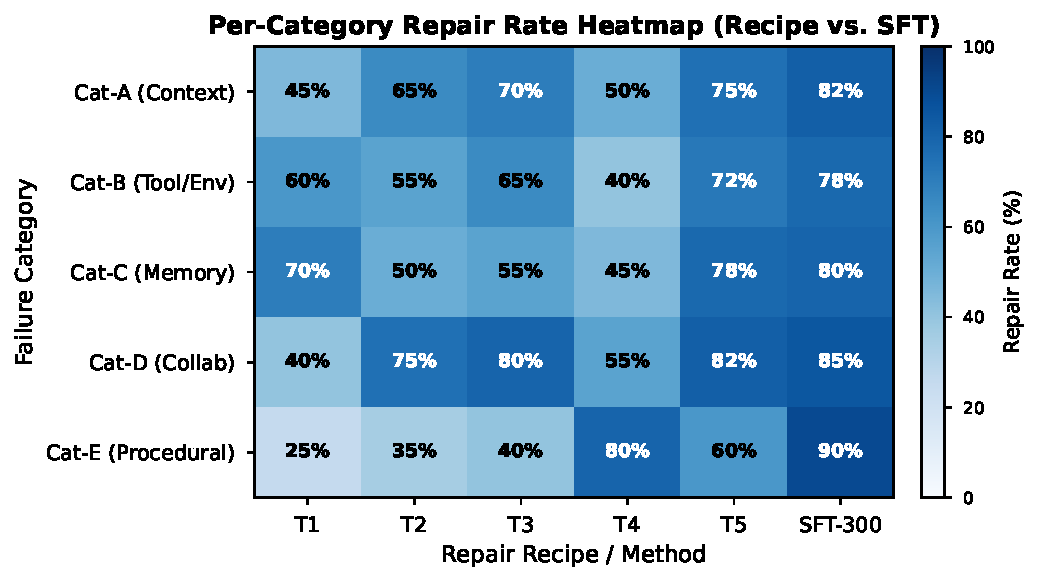
\includegraphics[width=\linewidth]{figs/category_repair_heatmap.pdf}
    \caption{Per-category repair rate heatmap for recipes T1--T5 and SFT-300 (mock data). Darker = higher repair rate. Cat.~E is hardest to repair without SFT.}
    \label{fig:repair-heatmap}
  \end{subfigure}
  \hfill
  \begin{subfigure}[b]{0.48\linewidth}
    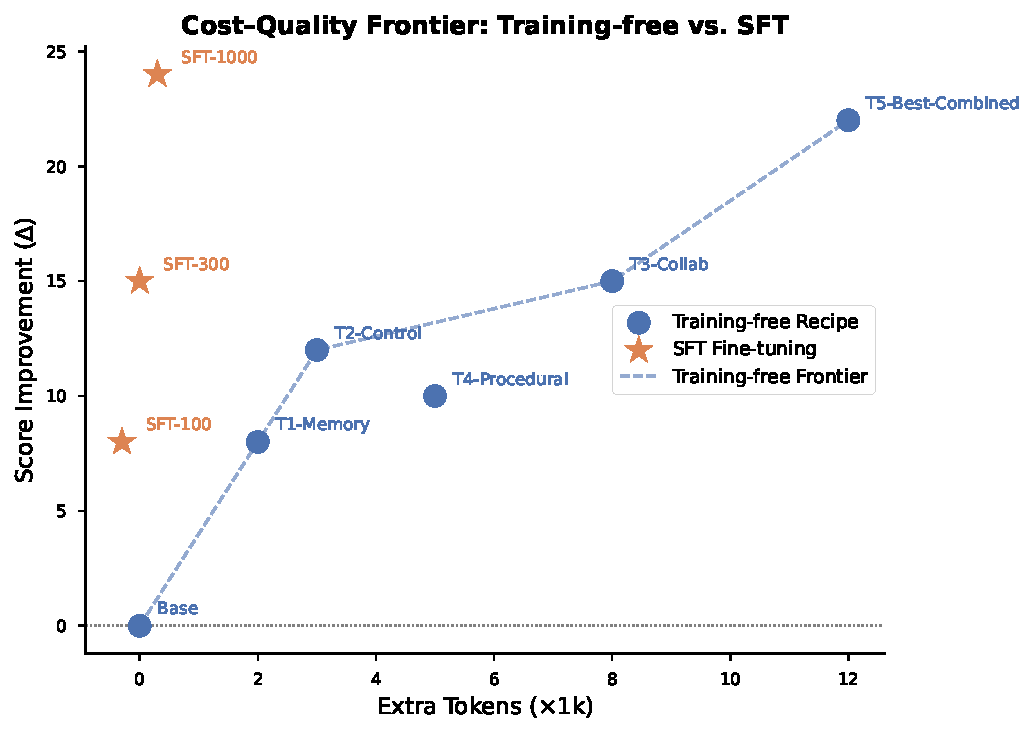
\includegraphics[width=\linewidth]{figs/cost_quality_frontier.pdf}
    \caption{Cost--quality frontier: extra tokens vs.\ score improvement $\Delta$. Training-free recipes (blue circles) vs.\ SFT variants (orange stars).}
    \label{fig:cost-quality}
  \end{subfigure}
  \caption{Repair analysis (mock data; to be replaced with real evaluation results). Left: per-category repair rates show T1--T3 are strongest on Cat.~C and Cat.~D; Right: SFT achieves higher $\Delta$ at zero token overhead but requires training.}
  \label{fig:repair-analysis}
\end{figure}

\section{Related Work}
\label{sec:related}
We situate our work at the intersection of three research areas.

\textbf{Agent evaluation and diagnosis.} Prior work on agent evaluation has focused on building comprehensive benchmarks~\citep{liu2023benchmarking,zheng2023judging} and measuring aggregate performance. We differ by diagnosing \emph{why} agents fail, building a structured taxonomy that enables per-category repair analysis. The closest prior work is \citet{zeng2024token}, which studies step-level credit assignment in DPO, and \citet{lai2024step} which proposes Step-DPO for redistributing preference weights to critical steps. Both focus on training-based credit assignment, while we focus on inference-time repair of structurally diagnosed failure categories.

\textbf{Training-free agent improvement.} Several works have proposed inference-time strategies for improving agents, including memory-augmented agents~\citep{le2022memory}, planner-executor splits~\citep{yao2023react}, and multi-agent collaboration~\citep{li2023multiagent}. We differ by systematically comparing these strategies against each other and against small-data SFT, using a shared taxonomy that clarifies which strategies repair which failure types. Prior comparisons~\citep{rporto2024agentrecipes} are conducted without a failure taxonomy and without controlled SFT baselines, making it difficult to identify the marginal value of each recipe.

\textbf{Failure analysis for LLMs.} Recent work has analyzed failure modes in LLMs for specific tasks such as math reasoning~\citep{tran2024understanding}, code generation~\citep{zhang2024debugging}, and tool use~\citep{patil2024evaluating}. We contribute a general failure taxonomy for multi-step agents that is benchmark-agnostic, with validation through a planned inter-annotator agreement study, and designed to be actionable for repair. Our taxonomy is related to but distinct from cognitive error taxonomies for humans~\citep{stanovich2011robot}.

\textbf{Small-data fine-tuning.} The question of how much data is needed for effective fine-tuning has been studied in domain adaptation~\citep{chen2021evaluate,zheng2023judging} and more recently in instruction tuning~\citep{zhou2024data}. We contribute a planned empirical study specifically focused on the interaction between SFT data scale and failure category, testing the hypothesis that category E (skill utilization deficiency) is the primary beneficiary of training and that the scaling curve has a threshold between 300 and 1,000 samples.

\section{Conclusion}
\label{sec:conclusion}
We presented a preliminary unified study of diagnosing and repairing failures in OpenClaw-like agents. Our contributions span three layers:

\begin{enumerate}[leftmargin=2em, itemsep=1pt]

  \item \textbf{Evaluation harness.} We built a reproducible evaluation protocol that pins benchmark versions, task splits, and evaluation protocols, enabling rigorous paired comparisons across repair strategies. We evaluate two benchmarks (PinchBench: 23 tasks; AgentBench-OpenClaw: 40 tasks) using the nanobot OpenClaw agent runtime.

  \item \textbf{Failure taxonomy.} We defined a five-class failure taxonomy (A: task understanding, B: tool grounding, C: memory/state, D: verification, E: skill utilization) informed by failure case analysis. Our initial analysis identifies structural failure patterns: E-type failures (ineffective skill utilization) account for 13--17\% of PinchBench tasks; the memory domain on AgentBench-OC consistently scores 50.0 across all model checkpoints, indicating a structural C-type failure.

  \item \textbf{Repair study (ongoing).} We design four training-free recipes and a small-data SFT protocol based on the observed failure patterns. Experimental evaluation of these repair strategies is planned as the next phase.

\end{enumerate}

Our central preliminary finding is that agent failures are not uniformly random but cluster into interpretable structural categories. E-type failures (skill utilization deficiency) require targeted interventions such as skill-activation prompting (T4b) or procedural knowledge injection (T4a); A-type and B-type failures show potential for prompting-based repair. Future work will complete the systematic repair evaluation to determine which failure categories respond to which repair strategy at what cost.

\section{Limitations}
\label{sec:limitations}

Our study has several limitations:

\begin{enumerate}[leftmargin=2em, itemsep=1pt]

  \item \textbf{Preliminary evaluation.} The systematic repair study (T1--T5 recipes, SFT conditions) has not yet been conducted. Conclusions about repair effectiveness are based on failure case analysis and design rationale, not empirical results.

  \item \textbf{Single base model.} All experiments use the doubao-seed-1.8 model. The failure taxonomy and repair effectiveness may vary for different base models. Validation on additional base models is needed.

  \item \textbf{Two benchmarks.} Our benchmark suite contains two benchmarks. The category distribution and repair rates may differ on other agent benchmarks. Future work should extend evaluation.

  \item \textbf{Informal annotation.} Failure categorization is based on case analysis by the authors, not formal annotation with inter-annotator agreement. A full annotated failure corpus is planned.

  \item \textbf{Evaluation variance.} On PinchBench, we observe substantial variance across runs (0.058 to 0.847 overall score on the same endpoint), likely due to API variability. This limits the sensitivity of score comparisons below 5 pp.

  \item \textbf{SFT data pipeline not yet built.} Trajectory correction, quality verification, and training pipelines are designed but not yet executed. SFT results are predictions based on the observed failure patterns, not empirical measurements.

\end{enumerate}


% ==================== References ====================
\bibliography{refs/references}
\bibliographystyle{acl_natbib}

% ==================== Appendix ====================
\appendix
\onecolumn

% ==================== Appendix Content ====================
\section{Per-Benchmark Detailed Results}
\label{app:per-benchmark}

Table~\ref{tab:per-benchmark} will report the paired delta ($\Delta$, in pp) and negative interference rate (NIR, \%) for each condition on each individual benchmark, complementing the per-benchmark results in Table~\ref{tab:pinchbench-results} and Table~\ref{tab:agentbench-results}.

\textbf{Note:} This table will be populated upon completion of the systematic repair evaluation (T1--T5 recipes and SFT conditions). The planned experimental design is described in \S\ref{sec:harness:conditions}. The current paper only reports Base condition results on PinchBench (Table~\ref{tab:pinchbench-results}) and AgentBench-OpenClaw (Table~\ref{tab:agentbench-results}).

\begin{table}[h]
\centering
\caption{Per-benchmark test results: paired delta ($\Delta$, pp) and NIR (\%). Results will be reported separately for AgentBench-OC and PinchBench upon completion of the repair evaluation pipeline. [Placeholder --- to be filled]}
\label{tab:per-benchmark}
\resizebox{\linewidth}{!}{%
\begin{tabular}{lcccc}
\toprule
 & \multicolumn{2}{c}{AB-OC} & \multicolumn{2}{c}{PB} \\
\cmidrule(lr){2-3}\cmidrule(lr){4-5}
\textbf{Condition} & $\Delta$ & NIR & $\Delta$ & NIR \\
\midrule
Base & 0.0 & 0.0\% & 0.0 & 0.0\% \\
+Memory & \emph{[TBD]} & \emph{[TBD]} & \emph{[TBD]} & \emph{[TBD]} \\
+Control & \emph{[TBD]} & \emph{[TBD]} & \emph{[TBD]} & \emph{[TBD]} \\
+Collab & \emph{[TBD]} & \emph{[TBD]} & \emph{[TBD]} & \emph{[TBD]} \\
+ProcSupport & \emph{[TBD]} & \emph{[TBD]} & \emph{[TBD]} & \emph{[TBD]} \\
+Memory+Control (T5) & \emph{[TBD]} & \emph{[TBD]} & \emph{[TBD]} & \emph{[TBD]} \\
SFT-100 & \emph{[TBD]} & \emph{[TBD]} & \emph{[TBD]} & \emph{[TBD]} \\
SFT-300 & \emph{[TBD]} & \emph{[TBD]} & \emph{[TBD]} & \emph{[TBD]} \\
SFT-1000 & \emph{[TBD]} & \emph{[TBD]} & \emph{[TBD]} & \emph{[TBD]} \\
\bottomrule
\end{tabular}}
\end{table}

\section{Ablation Study for Combined Recipe (T5)}
\label{app:ablation}

Table~\ref{tab:t5-ablation} will report CRR for each individual component (Memory alone, Control alone) and the combined T5 (+Memory+Control), on each failure category. This ablation is planned to be conducted on the test set.

\begin{table}[h]
\centering
\caption{Ablation of T5 (+Memory+Control) against individual components. CRR will be reported for each failure category upon completion of the evaluation. [Placeholder --- to be filled]}
\label{tab:t5-ablation}
\resizebox{0.8\linewidth}{!}{%
\begin{tabular}{lccccc}
\toprule
\textbf{Condition} & \textbf{A} & \textbf{B} & \textbf{C} & \textbf{D} & \textbf{E} \\
\midrule
+Memory & \emph{[TBD]} & \emph{[TBD]} & \emph{[TBD]} & \emph{[TBD]} & \emph{[TBD]} \\
+Control & \emph{[TBD]} & \emph{[TBD]} & \emph{[TBD]} & \emph{[TBD]} & \emph{[TBD]} \\
+Memory+Control (T5) & \emph{[TBD]} & \emph{[TBD]} & \emph{[TBD]} & \emph{[TBD]} & \emph{[TBD]} \\
\bottomrule
\end{tabular}}
\end{table}

\section{SFT Data Construction Details}
\label{app:sft-data}

For the SFT training data construction, corrected trajectories will be generated by prompting GPT-4o with the following template:

\medskip
\fbox{
\begin{minipage}{0.95\linewidth}
\textbf{System:} You are an expert agent that always produces correct trajectories. Given the task below, generate the correct sequence of actions and tool calls that leads to the gold answer. \\
\textbf{User:} Task: [task description] \\
Gold Answer: [gold answer] \\
Agent Trajectory (failed): [original trajectory] \\
Please generate the corrected trajectory with explanations.
\end{minipage}
}
\medskip

\textbf{Verification:} SFT training is planned as the next phase. Trajectory quality verification protocol (including human spot-checks of corrected trajectories) is planned as part of the SFT data construction pipeline.

\section{Annotation Protocol Details}
\label{app:annotation}

Formal failure annotation with inter-annotator agreement measurement is planned as part of the complete evaluation pipeline. The planned protocol follows the two-phase design in \S\ref{sec:taxonomy:annotation}: Phase 1 (pilot) with 60 failure traces and Phase 2 (formal) with 140 additional cases, targeting Cohen's $\kappa \ge 0.70$.

\section{Additional Baseline Details}
\label{app:baselines}

\textbf{Human ceiling:} Human expert evaluation on PinchBench and AgentBench-OC is planned but not yet conducted. This will provide an upper-bound reference for ceiling effect analysis.

\textbf{Inter-condition correlation:} Pearson correlation of paired deltas across conditions is planned as part of the full evaluation. This analysis will confirm that conditions targeting different failure categories capture distinct repair mechanisms.


\end{document}
